%%%%%%%%%%%%%%%%%%%%%%%%%%%%%%%%%%%%%%%%%
% baposter Landscape Poster
% LaTeX Template
% Version 1.0 (11/06/13)
%
% baposter Class Created by:
% Brian Amberg (baposter@brian-amberg.de)
%
% This template has been downloaded from:
% http://www.LaTeXTemplates.com
%
% License:
% CC BY-NC-SA 3.0 (http://creativecommons.org/licenses/by-nc-sa/3.0/)
%
%%%%%%%%%%%%%%%%%%%%%%%%%%%%%%%%%%%%%%%%%

%----------------------------------------------------------------------------------------
%	PACKAGES AND OTHER DOCUMENT CONFIGURATIONS
%----------------------------------------------------------------------------------------

\documentclass[landscape,a0paper,fontscale=0.3]{baposter} % Adjust the font scale/size here

\usepackage{float} % Required for multiple columns
\usepackage{placeins}
\usepackage{stfloats}
\usepackage[utf8]{inputenc}
\usepackage[T1]{fontenc}
\usepackage[english]{babel}

\usepackage{tabu}
\usepackage{tabularx}
\usepackage{booktabs, hhline}
\usepackage{subfig}
\usepackage{graphicx} % Required for including images
\graphicspath{{figures/}} % Directory in which figures are stored
\usepackage{graphicx}
\usepackage{amsmath} % For typesetting math
\usepackage{amssymb} % Adds new symbols to be used in math mode

\usepackage{booktabs} % Top and bottom rules for tables
\usepackage{enumitem} % Used to reduce itemize/enumerate spacing
\usepackage{palatino} % Use the Palatino font
\usepackage[font=small,labelfont=bf]{caption} % Required for specifying captions to tables and figures

\usepackage{multicol} % Required for multiple columns
\setlength{\columnsep}{1.5em} % Slightly increase the space between columns
\setlength{\columnseprule}{0mm} % No horizontal rule between columns
\selectcolormodel{cmyk}

\usepackage{tikz} % Required for flow chart
\usetikzlibrary{shapes,arrows} % Tikz libraries required forand Hongyu Liu and Tianyi Liu and Zhiqiang Lin and Tongping Liu the flow chart in the template

\newcommand{\compresslist}{ % Define a command to reduce spacing within itemize/enumerate environments, this is used right after \begin{itemize} or \begin{enumerate}
\setlength{\itemsep}{1pt}
\setlength{\parskip}{0pt}
\setlength{\parsep}{0pt}
}

\definecolor{darkgreen}{cmyk}{0.2394,0.0000,0.2394,0.2627}
\definecolor{orange}{cmyk}{0.0000,0.7294,1.0000,0.0000} 
\definecolor{floralwhite}{cmyk}{0.0000,0.0196,0.0588,0.0000}
\definecolor{gray}{cmyk}{0.0000,0.0000,0.0000,0.0392}
\definecolor{lightgreen}{cmyk}{0.7554,0.0000,0.7554,0.4549}
\definecolor{lightblue}{rgb}{0.145,0.6666,1} % Defines the color used for content box headers

\begin{document}

\begin{poster}
{
headerborder=closed, % Adds a border around the header of content boxes
colspacing=1em, % Column spacing
bgColorOne=white, % Background color for the gradient on the left side of the poster
bgColorTwo=white, % Background color for the gradient on the right side of the poster
borderColor=lightblue, % Border color
headerColorOne=lightblue, % Background color for the header in the content boxes (left side)
headerColorTwo=green, % Background color for the header in the content boxes (right side)
headerFontColor=black, % Text color for the header text in the content boxes
boxColorOne=white, % Background color of the content boxes
textborder=roundedleft, % Format of the border around content boxes, can be: none, bars, coils, triangles, rectangle, rounded, roundedsmall, roundedright or faded
eyecatcher=true, % Set to false for ignoring the left logo in the title and move the title left
headerheight=0.1\textheight, % Height of the header
headershape=roundedright, % Specify the rounded corner in the content box headers, can be: rectangle, small-rounded, roundedright, roundedleft or rounded
headerfont=\Large\bf\textsc, % Large, bold and sans serif font in the headers of content boxes
%textfont={\setlength{\parindent}{1.5em}}, % Uncomment for paragraph indentation
linewidth=2pt % Width of the border lines around content boxes
}
%----------------------------------------------------------------------------------------
%	TITLE SECTION 
%----------------------------------------------------------------------------------------
%
{
    
\includegraphics[height=3em]{figures/logo_grenoble}    
} % First university/lab logo on the left
%
{
    \bf\large\ \textsc{GuaNary}: Efficient Buffer Overflow Detection In Virtualized Clouds Using Intel EPT-based Sub-Page Write Protection Support\vspace{0.3em}
} % Poster title \vspace{0.2em}
{
    \textsl{\small Stella Bitchebe$^{1}$, Yves Kone$^{2}$, Pierre Olivier$^{3}$, Jalil Boukhobza$^{4}$, Yérom-David Bromberg$^{5}$, Daniel Hagimont$^{2}$, Alain Tchana$^{6}$\\
    $^1$Université Côte d'Azur, $^2$University of Toulouse, $^3$University of Manchester, $^4$ENSTA Bretagne, $^5$University of Rennes, $^6$Grenoble INP}\\ 
    \vspace{0.15em} 
    
\includegraphics[height=.9em]{figures/eurosys_23} %\vspace{0.2em}
    \hspace*{.3mm}
    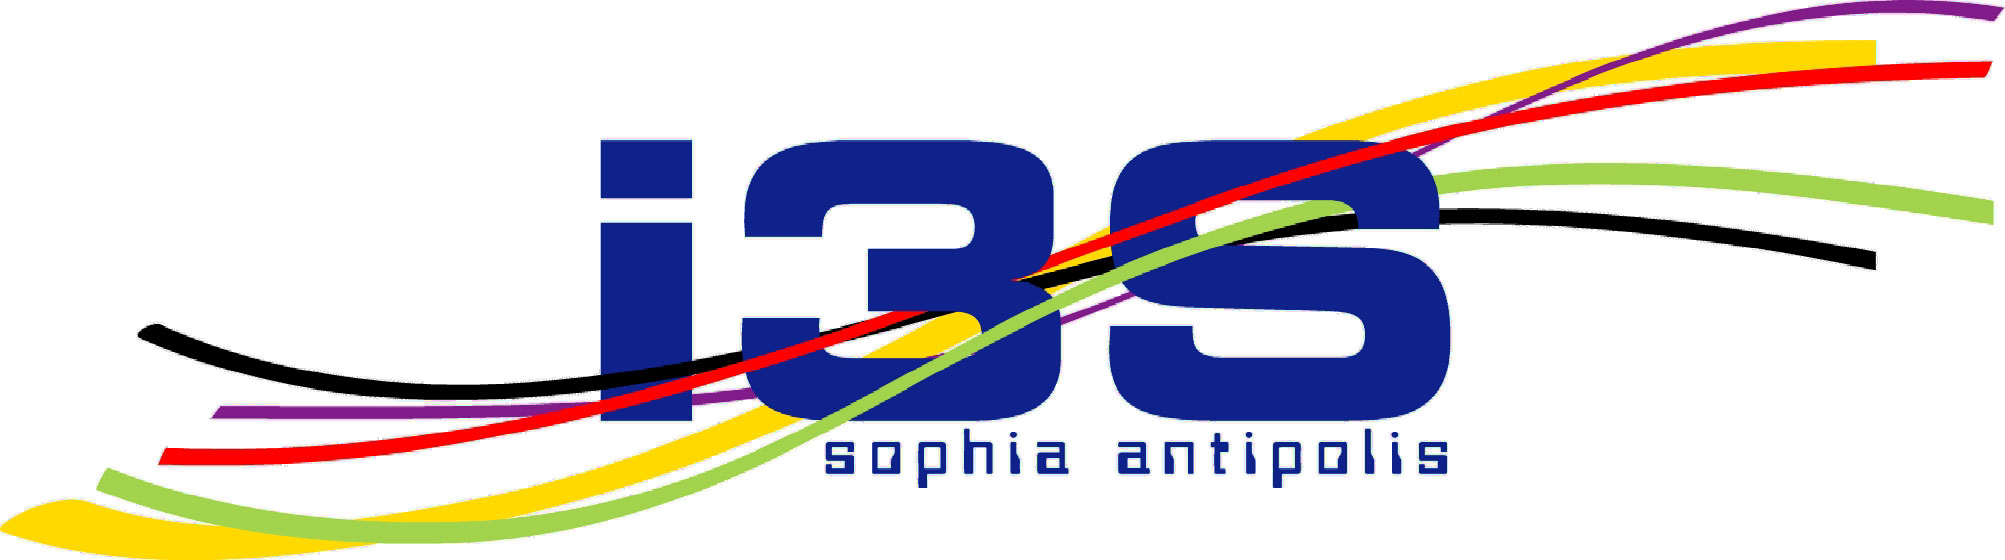
\includegraphics[height=1.7em]{figures/I3S}
} 
{
    
\includegraphics[height=4em]{figures/irit2}
}
%----------------------------------------------------------------------------------------
%	CTX & MOTIV
%----------------------------------------------------------------------------------------

\headerbox{1. Context and Motivation}{name=ctxmotiv,column=0,span=2}
{
    \begin{itemize}
        \item Buffer overflow was reported as the top vulnerability in 2022, according to the CWE (Common Weakness Enumeration)~\cite{top25}.
        \item Secure Allocators (e.g., Slimguard~\cite{slimguard}, Guarder~\cite{guarder}, etc.) generally use \emph{safety guards} located after a buffer to prevent and detect overflows.
        \item State-of-the-art safety guards: 
            \begin{itemize}
                \item \textcolor{blue}{\bf Canary}: 1-byte magic values checked to detect overflow => Modest memory overhead + Asynchronous detection (see Figure~\ref{fig:cn-gp-gn}).
                \item \textcolor{blue}{\textbf{Guard Page}}: unmapped pages in the virtual address space that trigger a fault if the page is hit by an overflow => Significant memory overhead + Synchronous detection (see Figures~\ref{fig:cn-gp-gn} and~\ref{fig:waste-parsec-gp1}).
            \end{itemize}
    \end{itemize}

    \centering
    \begin{minipage}[t]{.48\linewidth}
        \centering 
        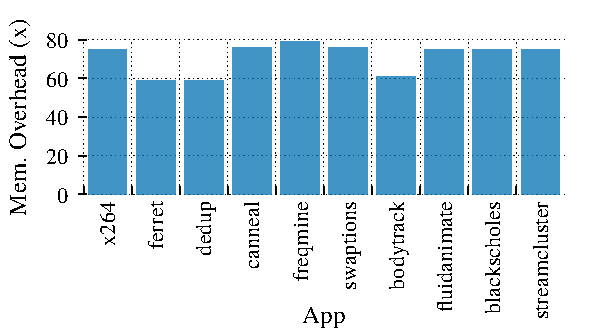
\includegraphics[width=.7\columnwidth]{figures/waste1}
        \captionof{figure}{Memory over-consumption that Slimguard would incur for PARSEC applications if all the allocated buffers are placed at the boundary of a guard page (worse case).}
        \label{fig:waste-parsec-gp1}		
    \end{minipage}
    \hfill
    \begin{minipage}[t]{.48\linewidth}
        \centering 
        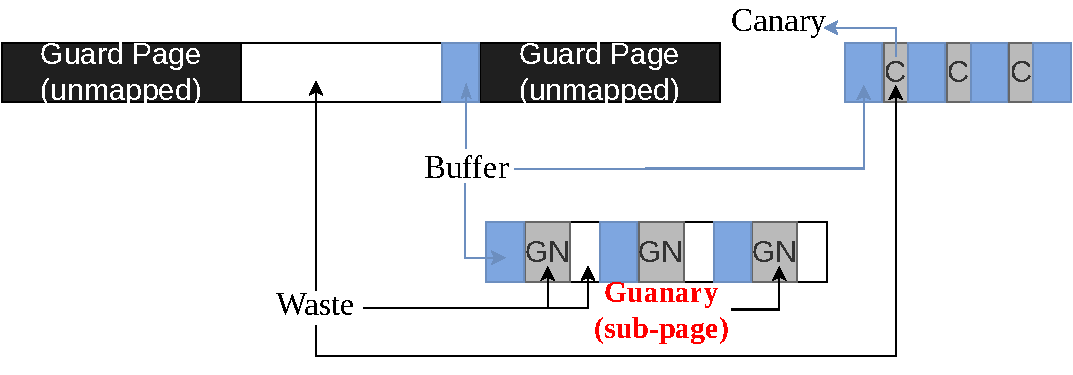
\includegraphics[width=.9\columnwidth]{figures/cn-gp-gn}
        \captionof{figure}{Canary, Guard pages, and GuaNary illustration. For the two latter, buffers are aligned with the lower boundary of the (sub)page.}
        \label{fig:cn-gp-gn}		
    \end{minipage}
%\vspace{-4cm} % When there are two boxes, some whitespace may need to be added if the one on the right has more content
}


\headerbox{2. Dilemma: Synchronuous Dectection vs. Memory Overhead}{name=dilem, column=2, span=2}
{
    \begin{multicols}{2}
        \begin{itemize}
            \item \textcolor{blue}{Security distance}: for a vulnerable buffer \texttt{b}, the security distance is the number of bytes separating \texttt{b} from a safety guard. A zero security distance allows catching overflow attempts immediately. Protecting all the buffers with a zero security distance is not practical for most existing allocators, as it would result in considerable memory overhead (like in Figure~\ref{fig:waste-parsec-gp1}).
            \item \textcolor{blue}{Protection frequency}: \texttt{F} is called the protection frequency if a safety guard is placed after every \texttt{F}-allocated buffers. 
            \item Memory overhead is a real conundrum for users who sacrifice security for better
            memory utilization or vice versa. To this end, they can configure \texttt{F} for better memory consumption and security trade-off (See Figure~\ref{fig:waste-parsec-gpn}).
        \end{itemize}

        \vspace{-0.4cm}

        \centering
        \begin{minipage}[t]{\columnwidth}
            \centering 
            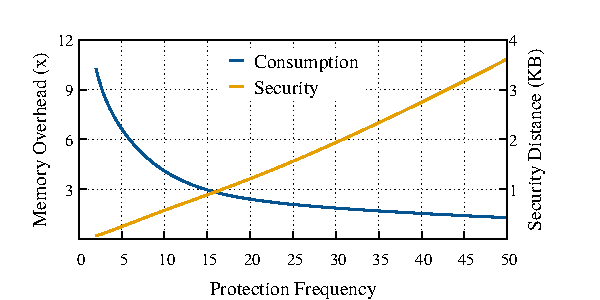
\includegraphics[width=.8\columnwidth]{figures/blackscholes}
            \captionof{figure}{Memory overhead and average security distances for PARSEC-\texttt{blackscholes} when varying the protection frequency from 2 to 50. The intersection between the two curves gives the optimal frequency, i.e., the one providing the best memory overhead and security trade-off. The allocator is Slimguard.}
            \label{fig:waste-parsec-gpn}		
        \end{minipage}

    \end{multicols}
}


%----------------------------------------------------------------------------------------
%	REFERENCES
%----------------------------------------------------------------------------------------

\headerbox{References}{name=references,column=0,above=bottom,span=3,boxColorOne=white}
{
    \begin{multicols}{2}
        \renewcommand{\section}[2]{\vskip 0.05em} % Get rid of the default "References" section title
        \nocite{*} % Insert publications even if they are not cited in the poster
        \scriptsize{ % Reduce the font size in this block
        \bibliographystyle{unsrt}
        \bibliography{sample} % Use sample.bib as the bibliography file
        }
    \end{multicols}
}

%----------------------------------------------------------------------------------------
%	RESULTS 
%----------------------------------------------------------------------------------------

\headerbox{4. GuarNary and LeanGuard}{name=guarnary,column=2,span=2,row=0,below=dilem,above=references}
{
    \begin{multicols}{2}      

        Using SPP, we introduce \textbf{\texttt{GuarNary}}, a novel type of safety guard that is midway between \texttt{Gua}rd page and ca\texttt{Nary}, thus providing the advantages of both solutions: synchronous buffer overflow detection and modest memory consumption (see Figure~\ref{fig:cn-gp-gn}).\\
        We also propose \textbf{\texttt{LeanGuard}} (see Figure~\ref{fig:leanguard-overview}), a software stack for \texttt{GuarNary} usage from inside virtual machines by new secure allocators.

        Figure~\ref{fig:mem-eval} shows that for the same number of protected buffers, LeanGuard consumes 8.3$\times$ less memory than SlimGuard. Further, for the same memory consumption, LeanGuard allows protecting 25$\times$ more buffers than SlimGuard.

        \begin{minipage}[t]{\columnwidth}
            \centering
            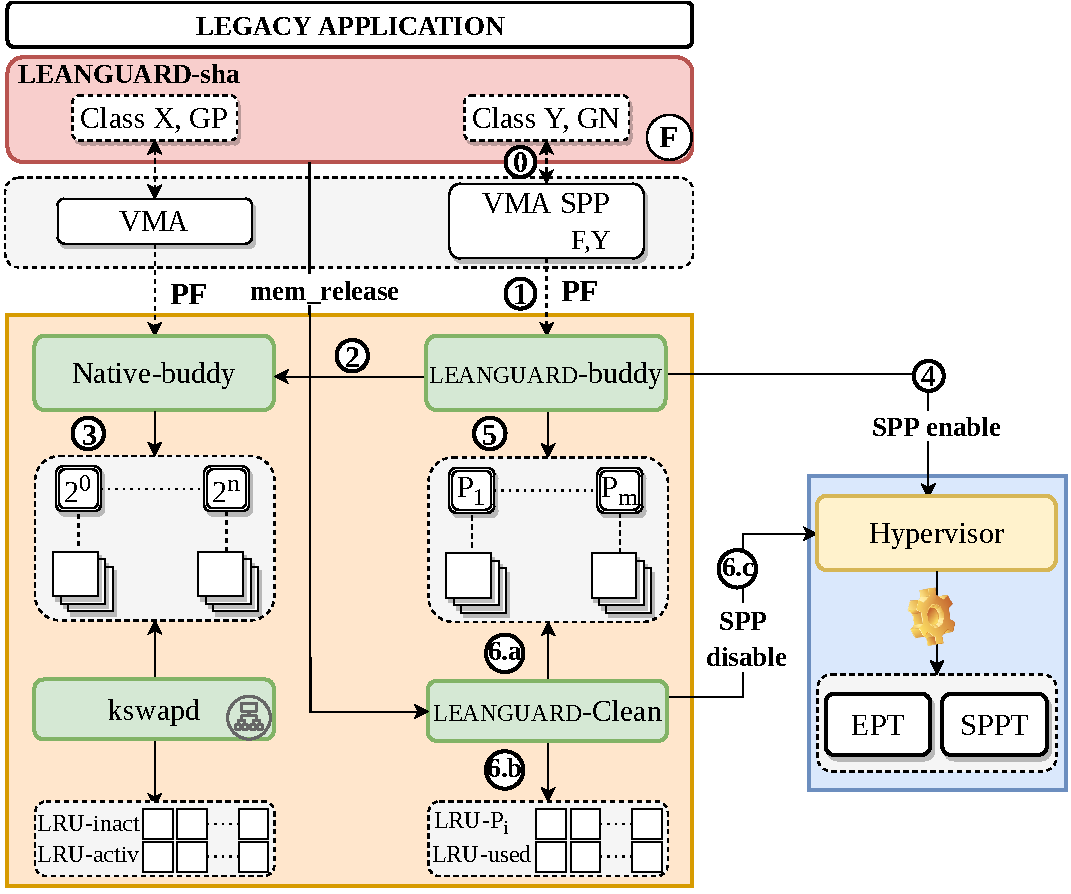
\includegraphics[width=.75\columnwidth]{figures/overview}
            \vspace*{-3.2mm}
            \captionof{figure}{Architecture of LeanGuard.} 
            \label{fig:leanguard-overview}      
        \end{minipage}
        
    \end{multicols}
    \vspace*{-2mm}
    \begin{minipage}[t]{\columnwidth}
        \centering
        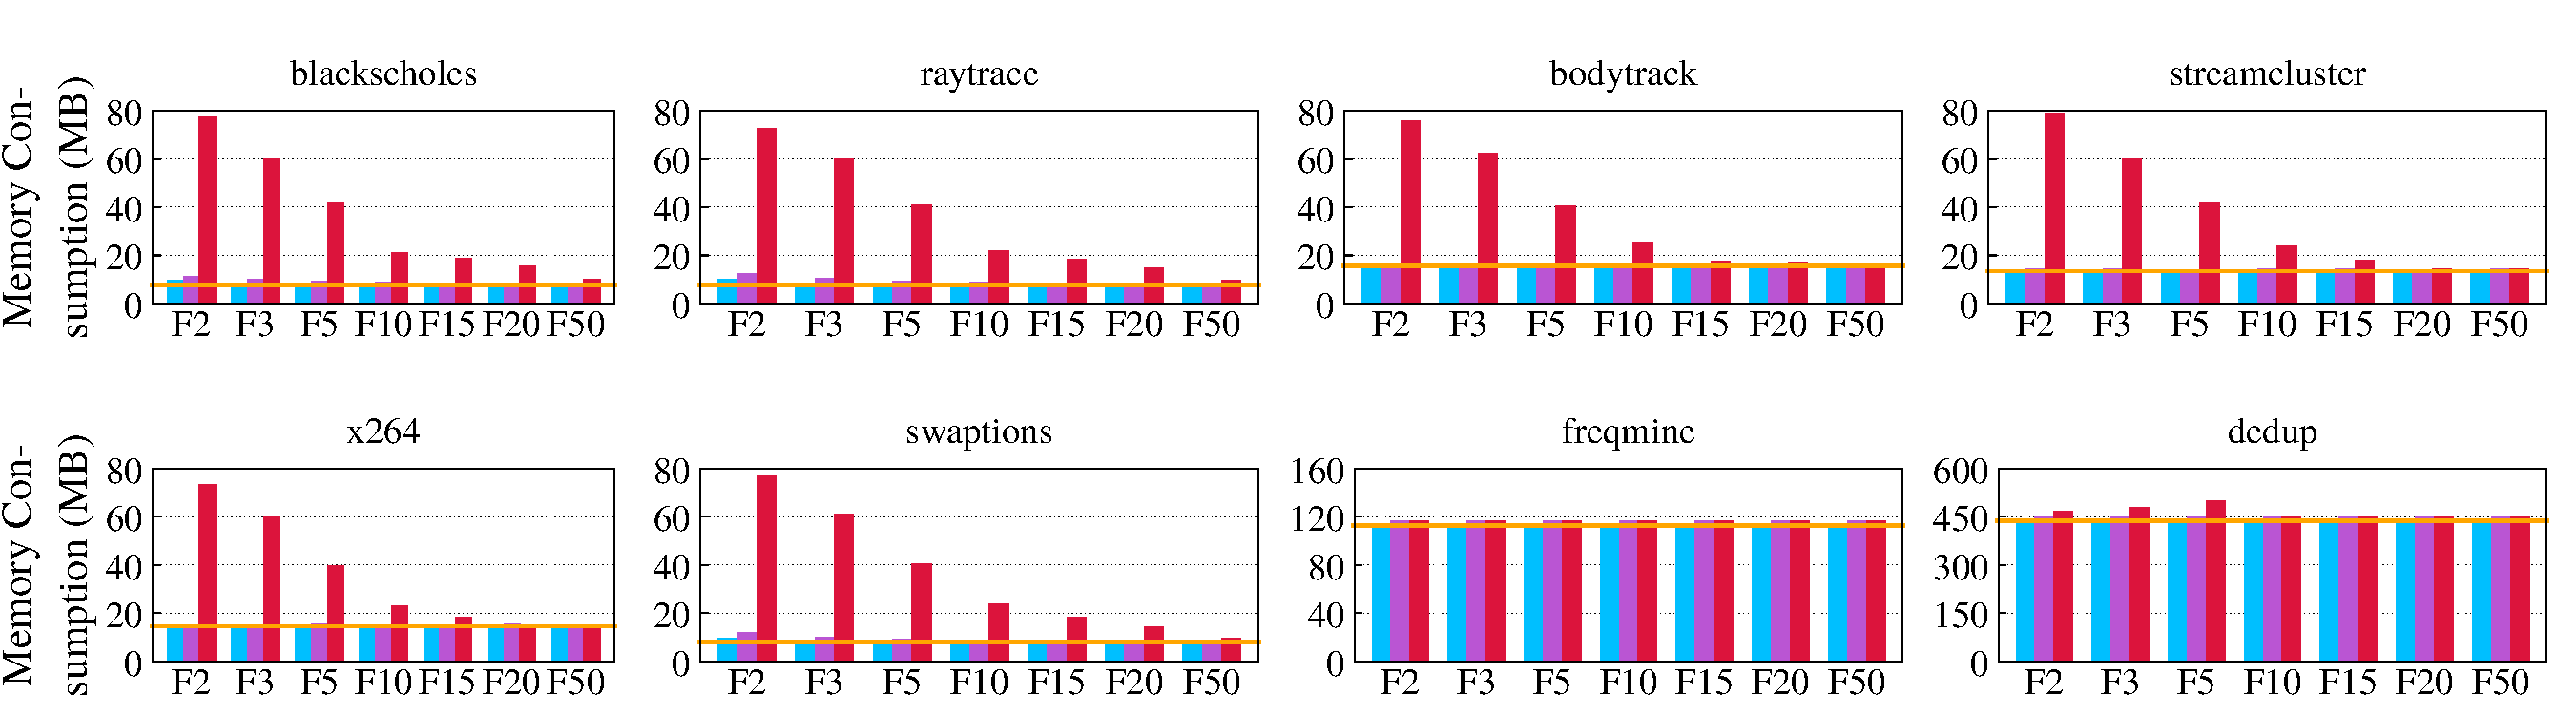
\includegraphics[width=.75\columnwidth]{figures/wss2}
        \vspace*{-4mm}
        \captionof{figure}{Memory consumption of each allocator configuration for PARSEC applications while varying the protection frequency.} 
        \label{fig:mem-eval}      
    \end{minipage}
}


%----------------------------------------------------------------------------------------
%	CONTACT INFORMATION
%----------------------------------------------------------------------------------------
\headerbox{Contact}{name=contact,column=3,aligned=references,above=bottom,boxColorOne=white}{ % This block is as tall as the references block

\begin{description}\compresslist
\small{
    \item
    \item bitchebe@i3s.unice.fr
    \item 
    \item alain.tchana@grenoble-inp.fr
    \item 
}
\end{description}
}

%----------------------------------------------------------------------------------------
%	CONTRIB
%----------------------------------------------------------------------------------------


%----------------------------------------------------------------------------------------
%	PROBLEM
%----------------------------------------------------------------------------------------

% \headerbox{Probl\'ematique}{name=problem,column=1,below=spp,above=references}{ % This block's bottom aligns with the bottom of the conclusion block
% Le canari et la page de garde sont des solutions tr\'es utilis\'es et matures mais pr\'esentes cependant des inconv\'enients.
% \vspace{0.1cm}
% \newline
% \textbf{\textcolor{orange}{Le canari}}
% \begin{itemize}
% \vspace{-0.1cm}
%     \item \textbf{Surco\^ut m\'emoire raisonnable:} pour n buffer \`a prot\'eger, seulement n octets suppl\'ementaires sont n\'ecessaires.
%     \item \textbf{D\'etection peu efficace:} la d\'etection de d\'epassements est \textcolor{orange}{\textbf{asynchrone}} et \`a se fait au niveau logiciel.
% \end{itemize}
% \textbf{\textcolor{orange}{La page de garde}}
% \begin{itemize}
%     \vspace{-0.1cm}
%     \item \textbf{D\'etection synchrone:} elle se fait lors de la traduction d'adresse.
%     \item \textbf{Surco\^ut m\'emoire potentiellement tr\`es \'elev\'e:} pour prot\'eger N buffer il faut au minumum \textcolor{orange}{\textbf{N pages}}.
% \end{itemize}
% \begin{figure}[H]
%     \centering
%     \vspace{-0.6cm}
%     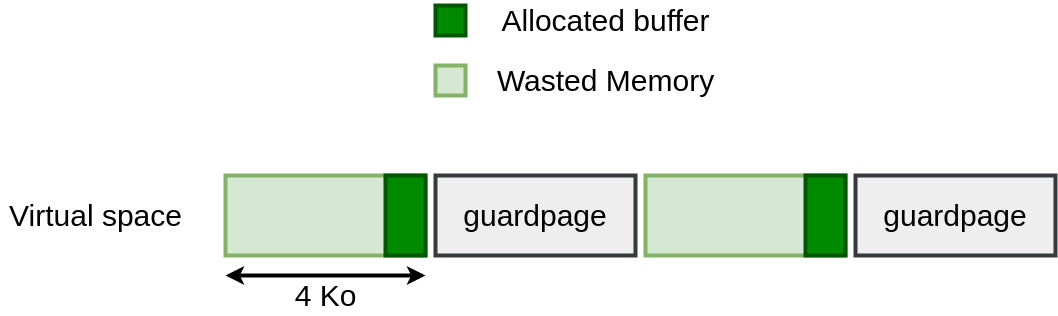
\includegraphics[width=0.9\linewidth]{guardpage_wasted}
%     \captionof{figure}{Sch\'ema de buffers prot\'eg\'es par des pages de garde. 
%     On voit ici que la m\'emoire consomm\'ee est de 8Ko (2 pages).}
% \end{figure}
% }

%----------------------------------------------------------------------------------------
%	MOTIV
%----------------------------------------------------------------------------------------

\headerbox{3. Intel SPP: Sub-Page Write Permission}{name=results2,column=0,below=ctxmotiv,above=references, span=2}
{ % This block's bottom aligns with the bottom of the conclusion block
    SPP~\cite{spp} is a recent Intel hardware virtualization feature that allows the hypervisor to write-protect guest’s memory at a sub-page (128B) granularity instead of 4KB (see Figure~\ref{fig:spp-walk}). SPP builds on top of the Extended Page Table (EPT)~\cite{ept}, introduced long ago to facilitate memory virtualization. 

    \begin{minipage}[t]{\linewidth}
        \centering
        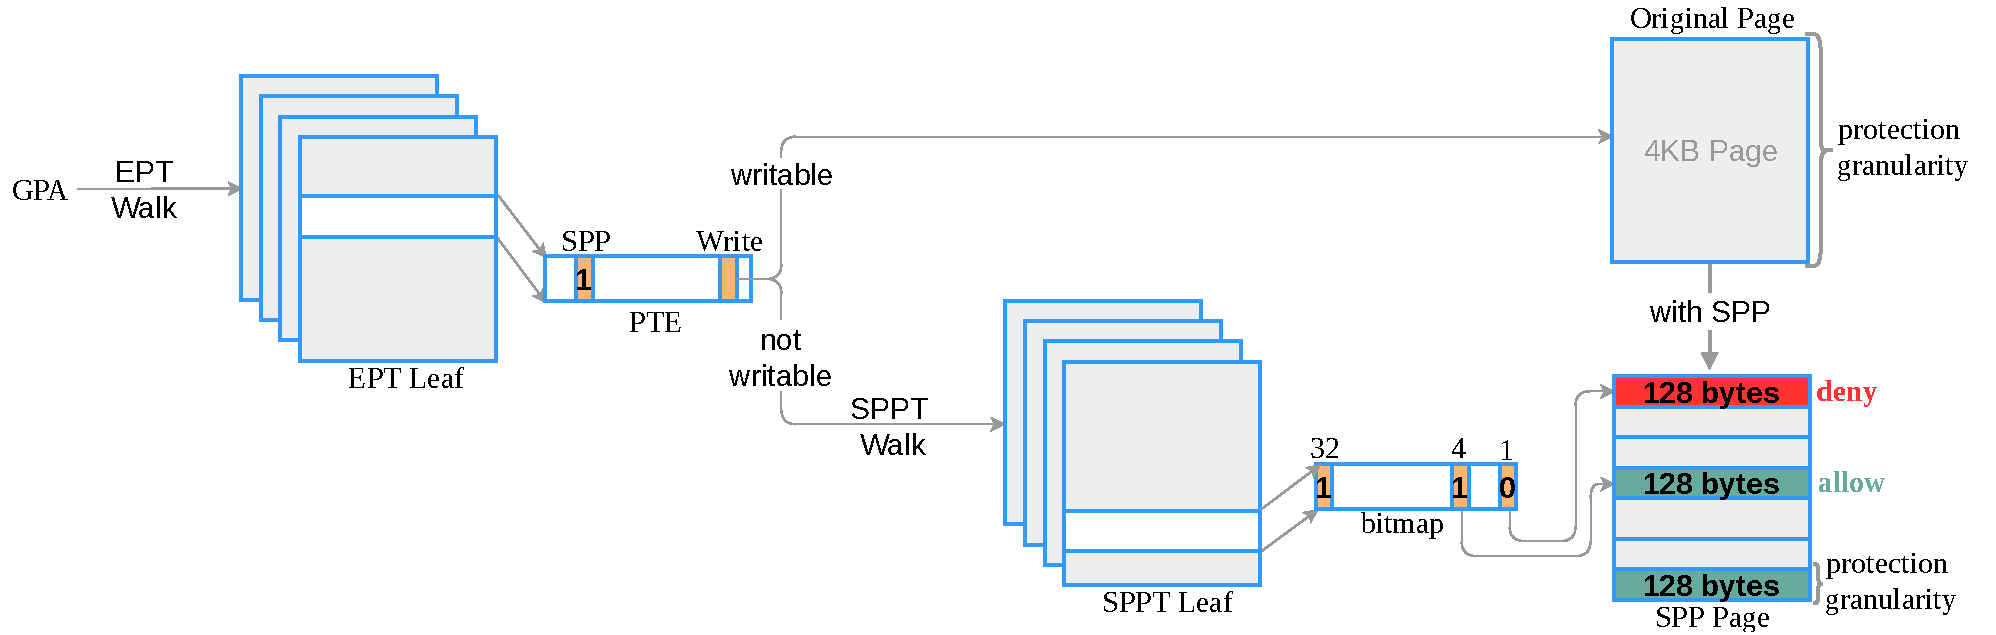
\includegraphics[width=.75\columnwidth]{figures/spp_walk}
        \vspace*{-2mm}
        \captionof{figure}{Overview of SPP functioning.} 
        \label{fig:spp-walk}      
    \end{minipage}    
}

%----------------------------------------------------------------------------------------

\end{poster}

\end{document}